\documentclass{standalone}
\usepackage{tikz}
\usepackage{verbatim}
\begin{document}
\pagestyle{empty}
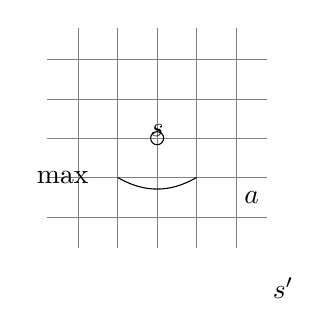
\begin{tikzpicture}

  % The graphic
  \draw[style=help lines,step=0.5cm] (-1.4,-1.4) grid (1.4,1.4);
  \node[draw,circle,scale=1/2] (s) at (0,0) {};
  \node at (0,0.1) {$s$};
  	% \node at (0.2, -0.5) {$\pi$};
   \node at (1.2, -0.75) {$a$};
   % \node[below = 2mm of b1] {$p$};
   %\node[below right = 1mm of b1] {$r$};
   \node at (1.6, -1.9) {$s'$};
	\node at (-1.2, -0.5) {max};
	\path[-] (-.5,-.5) edge[bend right=30] (.5, -.5);
\end{tikzpicture}
\end{document}